\documentclass{article}
\usepackage[utf8]{inputenc}
\usepackage[spanish]{babel}
\usepackage{pdfpages}
\usepackage{listings}
\usepackage{graphicx}
\usepackage{float}

\usepackage{mips}
\setlength{\parskip}{1ex plus 0.5ex minus 0.2ex}

\title{Trabajo Prático 0} 
\author{\\
  Agustin Alejandro Linari, \textit{Padrón Nro. 81.783}\\
  \textit{agustinlinari@gmail.com}\\
  \and
  Juan Ignacio López Pecora, \textit{Padrón Nro. 84.700}\\
  \textit{jlopezpecora@gmail.com}\\
  \and
  Pablo Daniel Sívori, \textit{Padrón: 84.026}\\
  \textit{sivoridaniel@gmail.com}\\
  \\
  \normalsize{2$^{\circ}$ Cuatrimestre de 2016}                           \\
  \normalsize{66.20 Organizacion de Computadoras}                  \\
  \normalsize{Facultad de Ingenieria, Universidad de Buenos Aires} \\
}

%\newcommand{\ip}[2]{(#1, #2)}
                             % Defines \ip{arg1}{arg2} to mean
                             % (arg1, arg2).

%\newcommand{\ip}[2]{\langle #1 | #2\rangle}
                             % This is an alternative definition of
                             % \ip that is commented out.

\begin{document}             % End of preamble and beginning of text.

\maketitle                   % Produces the title.

\begin{abstract}
En presente trabajo se diseña un programa en el lenguaje C que permite graficar el conjunto de Julia y sus vecindades para un polinomio cuadrático. 
\end{abstract}

\clearpage

\tableofcontents
\clearpage

\part{Desarrollo}

\section{Introduccion}

El objetivo del presente trabajo práctico es familiarizarse con las herramientas de software a utilizar durante el transcurso de la materia. Para ello implementaremos un programa en lenguaje C que dado ciertos parámetros de entrada se ocupará de generar una imagen en formato PGM del conjunto de Julia de un polinómio cuadrático. 
Finalmente compilaremos el programa en el emulador GXemul para poder obtener el código de instrucciones Mips32.

\section{Build}
El correspondiente informe se puede construir utilizando el make con la etiqueta doc la cual borra y genera el informe en formato pdf.

\section{Diseño e Implementación del Programa}
Para el desarrollo del programa se utilizó como base el pseudocódigo proporcionado en el enunciado del trabajo práctico. \ref{sec:enunciado}
Para su codificación en el lenguaje C, se necesitó crear un TDA complex para encapsular las operaciones con números complejos. Mediante la utilización de la libreria math, se desarrollaron funciones para las operaciones requeridas en el cómputo del algoritmo generador del fractal. Es decir, se implementaron la multiplicación, adición y módulo de complejos. También se agregó una función adicional que permite mapear cada uno de los pixels al punto del plano complejo correspondiente. 

El primer paso es dividir el plano complejo según la resolución. 

El ancho de cada división es el ancho del plano (w) dividido la resolución horizontal (x).

$\Delta$w = w/x

El alto de cada división es el alto del plano (h) dividido la resolución vertical (y).

$\Delta$h = h/y

El punto superior izquierdo del plano ($z_{0}$), se obtiene a partir del centro del plano (c).

Re($z_{0}$) = Re(c) - w/2

Im($z_{0}$) = Im(c) + h/2

Luego dado un pixel (i, j) se obtiene el z correspondiente.

Re(z) = Re($z_{0}$) + $\Delta$w/2 + $\Delta$w$\cdot$i

Im(z) = Im($z_{0}$) - $\Delta$h/2 - $\Delta$h$\cdot$j

En cuanto al formato de salida para la imagen, se utilizó el formato Plain PGM.

Los argumentos que llegan al programa se parsearon utilizando la librería getopt. 
El código fuente del programa se puede encontrar en el anexo \ref{sec:source}.

\section{Corridas de Programa}

\subsection{Ejemplos}

Primero realizamos la prueba de generar las dos imagenes que se daban de ejemplo en el enunciado. Para el primer caso generamos la imagen con los valores dados por defecto. Esta se puede ver en la carpeta test con el nombre uno.pgm.
Para la segunda imagen hacemos zoom sobre la región centrada en +0,282 − 0,01i, usando un rectángulo de 0,005 unidades de lado. Esta figura se puede ver en la carpeta test con el nombre dos.pgm.

\subsection{Pruebas}

Luego de verificar que el programa genera las imagenes correspondiente a los ejemplos, procedimos a ejecutar los casos de prueba. Para ello nos posicionamos en la carpeta raíz que contiene al archivo run-test.sh y luego realizamos la ejecución de este archivo  haciendo sh run-test.sh, retornando como output los resultados correspondientes a cada prueba.
A continuación detallamos los resultados de las pruebas realizadas.


\begin{enumerate}
   
    \item \textbf{Generación de una imagen de 1 punto de lado, centrada en el orı́gen del plano 	complejo.}\n

	Aquí se observa que el resultado del test es passed. Esto significa que paso la prueba satisfactoriamente.
	
	Para esto se uso el valor esperado expected1.pgm que se encuentra en la carpeta test.
    
    \item \textbf{Un punto que no pertenece al conjunto.}

	Aquí se observa que el resultado del test es passed. Esto significa que paso la prueba satisfactoriamente.    
	
	Para esto se uso el valor esperado expected2.pgm que se encuentra en la carpeta test.
	
    
    \item \textbf{Imagen imposible.}

	Aquí se observa que el resultado del test es passed. Esto significa que paso la prueba satisfactoriamente. 
	
	Para esto se uso el valor esperado expected3 que se encuentra en la carpeta test.   

	\item \textbf{Archivo de salida imposible.}    
	
	Aquí se observa que el resultado del test es passed. Esto significa que paso la prueba satisfactoriamente. 
	
	Para esto se uso el valor esperado expected4 que se encuentra en la carpeta test.
	
	\item \textbf{Coordenadas complejas imposibles.}   
	
	Aquí se observa que el resultado del test es passed. Esto significa que paso la prueba satisfactoriamente. 
	
	Para esto se uso el valor esperado expected5 que se encuentra en la carpeta test.
	
	\item \textbf{Argumentos de líneas de compando vacíos.}    
	
	Aquí se observa que el resultado del test es passed. Esto significa que paso la prueba satisfactoriamente. 
	
	Para esto se uso el valor esperado expected6 que se encuentra en la carpeta test.
    
\end{enumerate}


\clearpage

\part{Apendice}
\appendix


\section{Codigo fuente}\label{sec:source}
\definecolor{gray}{rgb}{0.5,0.5,0.5}
\lstset{%
  title=\lstname,
  language=C,
  basicstyle=\footnotesize,
  showspaces=false,
  showstringspaces=false,
  breaklines=true,
  commentstyle=\color{gray},
  numbers=left,
  numberstyle=\tiny\color{gray},
  numbersep=5pt,
  frame=single
}

\lstinputlisting{../src/complex.h}
\lstinputlisting{../src/complex.c}
\lstinputlisting{../src/app.c}

\clearpage

\lstset{%
  language=[mips]Assembler,       % the language of the code
  basicstyle=\footnotesize,       % the size of the fonts that are used for the code
  numbers=left,                   % where to put the line-numbers
  numberstyle=\tiny\color{gray},  % the style that is used for the line-numbers
  stepnumber=1,                   % the step between two line-numbers. If it's 1, each line 
                                  % will be numbered
  numbersep=5pt,                  % how far the line-numbers are from the code
  backgroundcolor=\color{white},  % choose the background color. You must add \usepackage{color}
  showspaces=false,               % show spaces adding particular underscores
  showstringspaces=false,         % underline spaces within strings
  showtabs=false,                 % show tabs within strings adding particular underscores
  frame=single,                   % adds a frame around the code
  rulecolor=\color{black},        % if not set, the frame-color may be changed on line-breaks within not-black text (e.g. commens (green here))
  tabsize=4,                      % sets default tabsize to 2 spaces
  captionpos=b,                   % sets the caption-position to bottom
  breaklines=true,                % sets automatic line breaking
  breakatwhitespace=false,        % sets if automatic breaks should only happen at whitespace
  title=\lstname,                 % show the filename of files included with \lstinputlisting;
                                  % also try caption instead of title
  keywordstyle=\color{blue},      % keyword style
  commentstyle=\color{green},     % comment style
  stringstyle=\color{red},      % string literal style
  escapeinside={\%*}{*)},         % if you want to add a comment within your code
  morekeywords={*}                % if you want to add more keywords to the set
}

\lstinputlisting{../MIPS32/complex.s}
\lstinputlisting{../MIPS32/app.s}

\clearpage

\section{Enunciado original}\label{sec:enunciado}
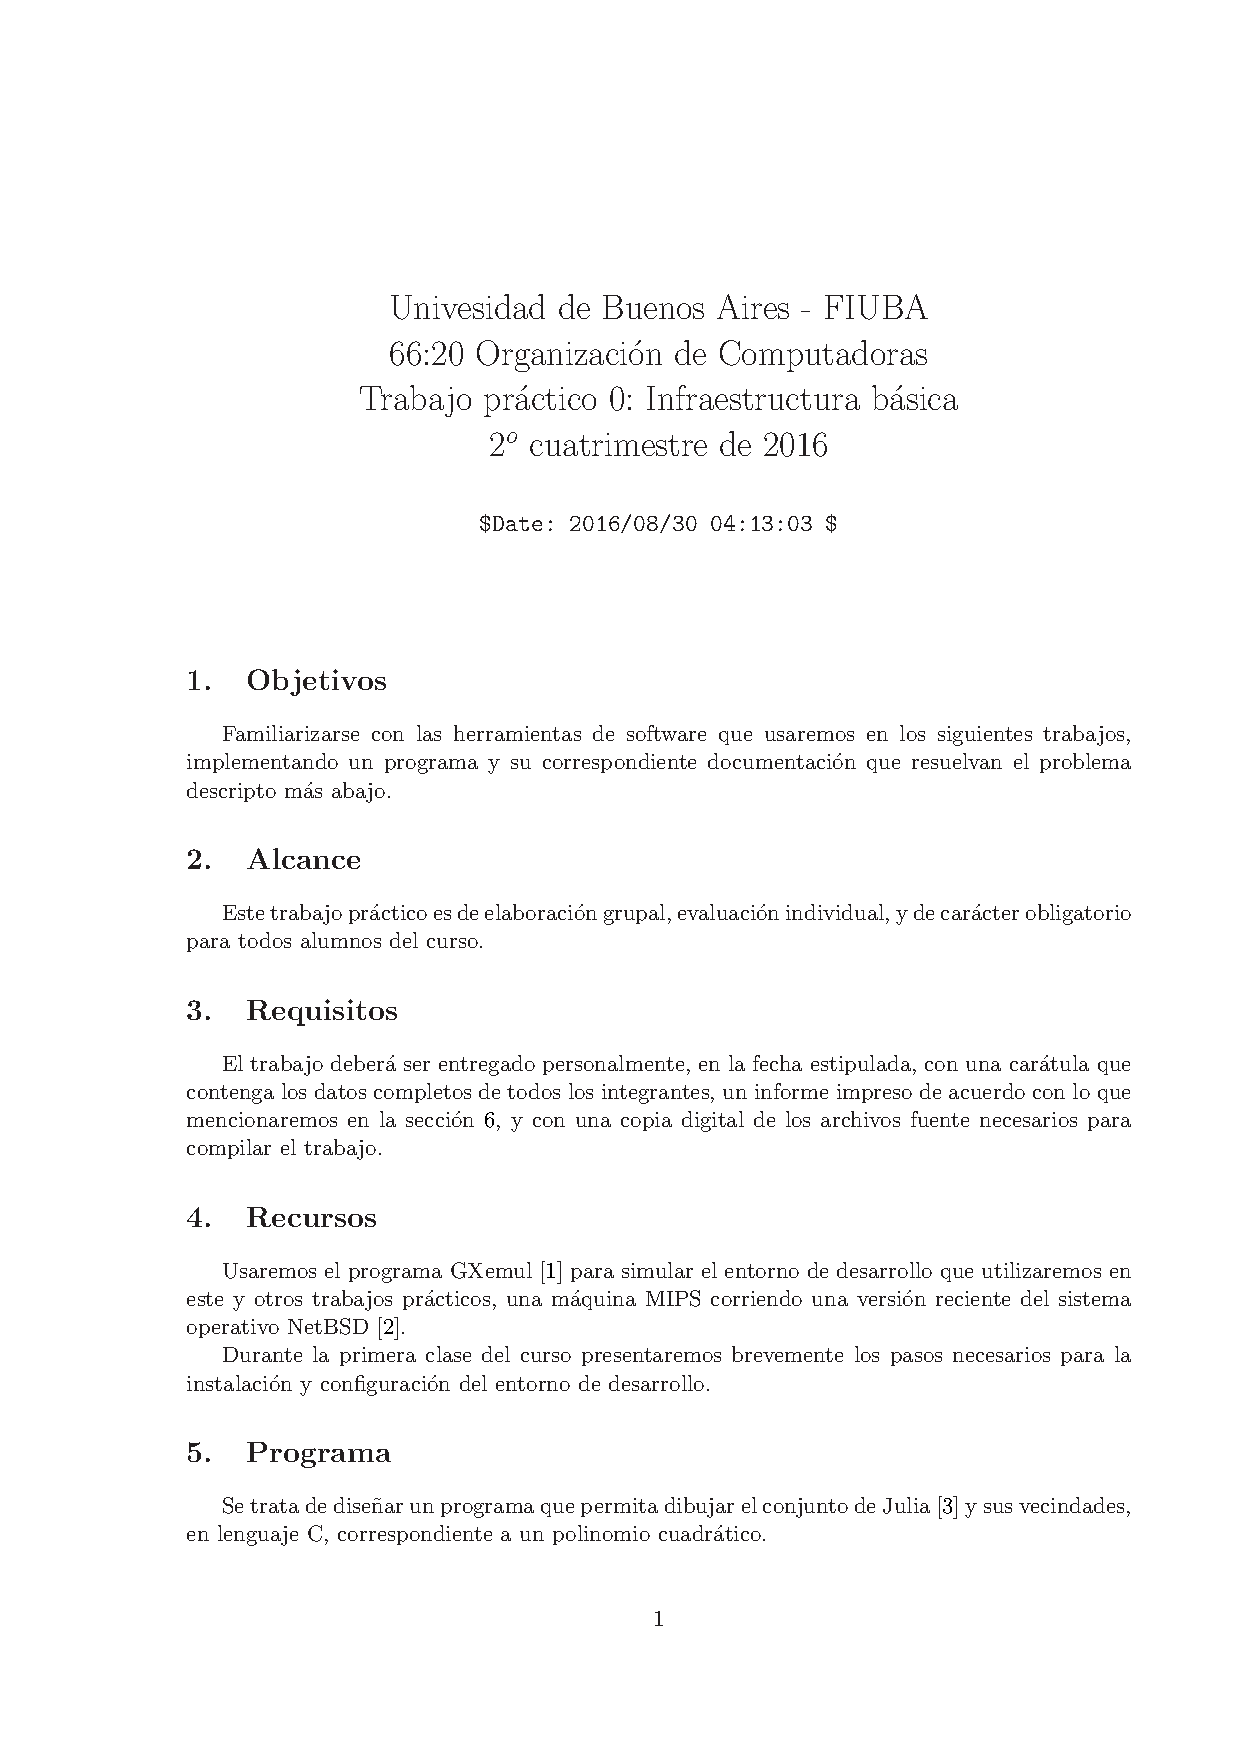
\includepdf[pages={-}]{tp0-2016-2q.pdf}

\end{document}               % End of document.
